\section{Analisi}
\subsection{Requisiti}

Il gruppo si pone come obiettivo quello di realizzare la trasposizione videoludica del gioco da tavolo Carcassonne. Si tratta di un gioco da 2 a 6 giocatori dove ognuno deve posizionare delle tessere e delle pedine con lo scopo di realizzare punti vittoria. Chi alla fine avrà totalizzato più punti vittoria verrà proclamato vincitore. Le tessere devono essere poste in maniera adiacente in modo che combacino tra di loro e formino strutture, ovvero strade, praterie, città o monasteri. Posizionando un seguace su una struttura, il giocatore ne prende la proprietà, guadagnandone poi i punti alla sua chiusura.

\begin{figure}[]
    {\includegraphics[]{images/Città.png}}

    \caption{Chiudere una città comporta l’assenza di parti non murate, facendo guadagnare al proprietario 2 punti per ogni tessera all'interno della città. Nel caso una tessera contenga uno stemma, allora varrà il doppio}
\end{figure}

\begin{figure}[]
    {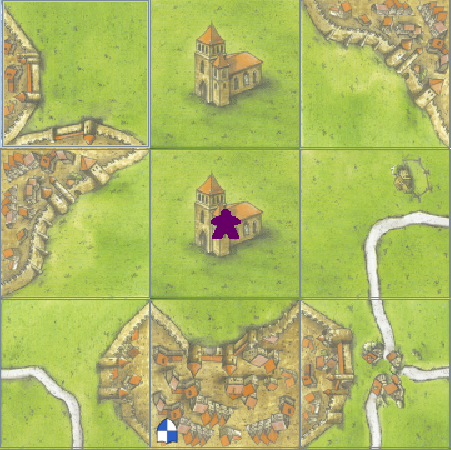
\includegraphics[]{images/MonasteroMeeple.png}}

    \caption{Chiudere un monastero comporta che questo sia circondato da 8 tessere, facendo guadagnare al proprietario 9 punti}
\end{figure}

\begin{figure}[]
    {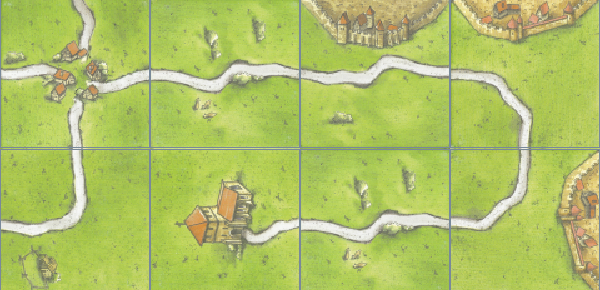
\includegraphics[]{images/Strada.png}}

    \caption{Chiudere una strada comporta la presenza di un incrocio o un’entrata ad un monastero/città da ambo i lati, facendo guadagnare al proprietario 1 punto per ogni tessera, estremi compresi}
\end{figure}

\subsection*{Requisiti funzionali}
Il gioco dovrà permettere ai giocatori che ne partecipano, ognuno identificato univocamente da nome e colore, di piazzare e ruotare tessere ed eventualmente posizionarvi sopra un seguace. E' necessario:

\begin{itemize}
\item Permettere il posizionamento delle tessere solo se posizionate in modo adiacente alle tessere già in campo ed esclusivamente nel caso in cui ogni lato della tessera corrente combaci con il lato della tessera vicina
\item Permettere la navigazione del campo di gioco
\item Permettere il posizionamento di seguaci solamente nella tessera appena piazzata appurato che non ci siano altri seguaci nella stessa struttura
\end{itemize}

Calcolo dei punteggi dei giocatori: ogni giocatore avrà il suo punteggio corrente che incrementerà ogni volta che durante il suo turo "chiuderà" una struttura seguendo le regole del gioco

ogni giocatore otterrà il suo punteggio finale sommando al suo punteggio corrente il punteggio ogni seguace ancora presente nel terreno quindi


\subitem i punteggi residui di ogni seguace posizionato in una struttura non "chiusa"

\subitem i punteggi ottenuti da ogni seguace posizionato in un prato seguendo le regole del gioco come nella figura 4

\begin{figure}[]
    %{\includegraphics[]{images/Prato.png}}

    \caption{Ogni prato è delimitato e rappresentato da ogni strada e città che lo circonda}
    
    % , ed è rappresentato dall'insieme di ogni tessera
    % Un prato è rappresentato dall'insieme di ogni sezione verde presente sulle tessere che ne delimitano i lati tramite strade e città}
\end{figure}

\begin{itemize}
\item Menù principale, con selezione numero giocatori
\end{itemize}
\begin{itemize}
\item Gestione turno del giocatore
\end{itemize}
\begin{itemize}
\item Gestione posizionamento pedine
\end{itemize}
\begin{itemize}
\item Calcolo delle posizioni valide per le tessere: ad ogni tentativo di posizionamento della tessera dovrà essere verificata la possibilità di effettuare l'azione. Si gestirà anche il caso in cui la tessera dovrà esssere obbligatoriamente scartata in quanto non esistono posti validi in cui in cui posizionarla
\end{itemize}
\begin{itemize}
\item Gestione della creazione o ampliamento di prati, città e strade
\end{itemize}

\subsection*{Requisiti non funzionali}
\begin{itemize}
\item Menù di pausa
\end{itemize}
\begin{itemize}
\item Visualizzazione grafica e dinamica dei seguaci rimanenti 
\end{itemize}
\begin{itemize}
\item Pannello per la scelta del colore del giocatore
\end{itemize}
\begin{itemize}
\item Decorazioni, sfondi e distanziamento fra i vari componenti grafici
\end{itemize}
\begin{itemize}
\item Supporto di espandibilità futura per l'implementazione di immagini di profilo dei giocatori
\end{itemize}
\begin{itemize}
\item Supporto per partecipare alla stessa partita da più interfacce
\end{itemize}
\begin{itemize}
\item Supporto per future espansioni con l'aggiunta di nuove tessere e seguaci
\end{itemize}

\subsection{Analisi e modello del dominio}
L'analisi e il modello di dominio di Carcassonne possono essere suddivisi in diversi componenti chiave, tra cui il tabellone di gioco, le tessere, i meeples e il sistema di punteggio.
\begin{itemize}
    \item Tabellone di gioco (Mappa): Il tabellone di Carcassonne rappresenta la regione di Carcassonne ed è composto da una serie di tessere che vengono posizionate sul tabellone durante il gioco. Il tabellone è suddiviso in diverse regioni, tra cui città, strade, campi e monasteri. Ognuna di queste regioni ha le proprie regole e il proprio sistema di punteggio, che aggiungono profondità e complessità al gioco.
    \item Le tessere (Tiles): Le tessere di Carcassonne rappresentano diversi tipi di terreno, tra cui città, strade, campi e monasteri. Queste tessere vengono estratte casualmente da una pila e devono essere posizionate sul tabellone di gioco in modo che corrispondano al tipo di terreno delle tessere circostanti. Ogni tessera ha le sue regole e il suo sistema di punteggio, che i giocatori devono seguire per massimizzare i loro punti.
    \item Meeples: I meeple sono i pezzi di gioco che i giocatori usano per controllare le diverse regioni del tabellone. 
    \item Sistema di punteggio: Il sistema di punteggio di Carcassonne si basa sul completamento di diverse regioni sul tabellone di gioco. Quando una città, una strada o un monastero vengono completati, il giocatore che ha il maggior numero di meeples su di essi ottiene i punti. Se più giocatori hanno meeples su un elemento completato, ognuno di loro ottiene i punti. Alla fine della partita, i giocatori ottengono punti anche per i loro contadini sui campi completati. Il giocatore con il maggior numero di punti alla fine del gioco è il vincitore.
\end{itemize}
Le difficoltà che il progetto mantiene sono sopratutto presenti nella parte grafica, non ancora ottimizzata a causa dell'utilizzo del framework grafico Java Swing.
